\subsection{Scenario 3: Growing Infrastructure}
\begin{figure}[H]
    \centering
    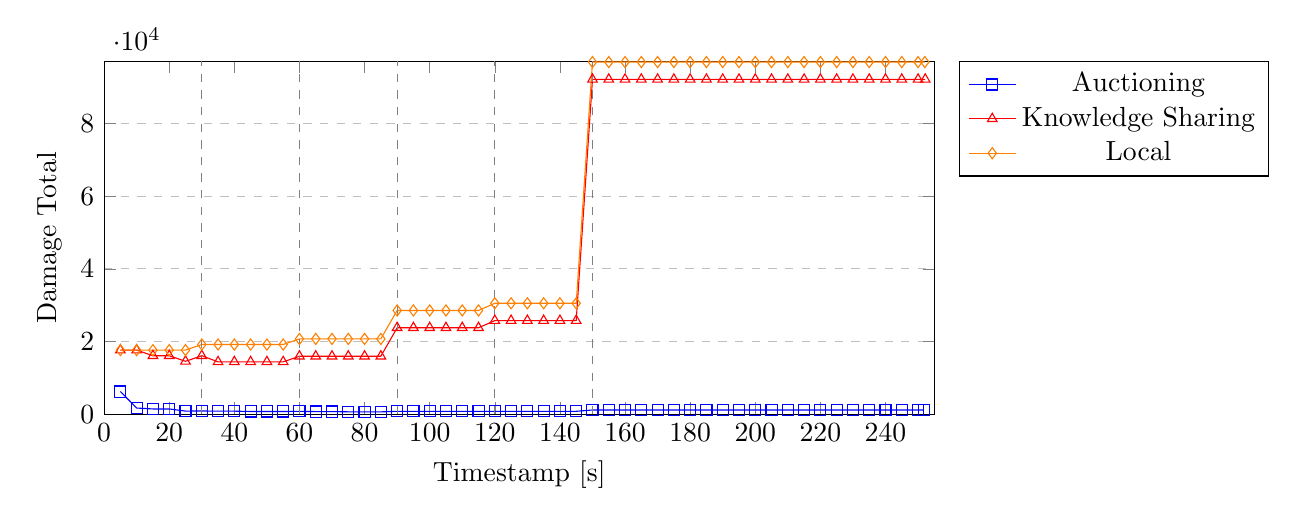
\begin{tikzpicture}
\begin{axis}[
    xlabel={Timestamp [s]},
    ylabel={Damage Total},
    xmin=0, xmax=255000,
    ymin=0, ymax=97097,
    legend pos=outer north east,
    ymajorgrids=true,
    grid style=dashed,
    width=\textwidth,
    height=0.5\textwidth,
    scaled x ticks=base 10:-3,
    xtick scale label code/.code={}
]

	\addplot[color=blue,mark=square] coordinates {
        (5000,6236.51)(10000,1693.70)(15000,1442.78)(20000,1442.78)(25000,857.00)(30000,882.24)(35000,830.70)(40000,830.70)(45000,747.92)(50000,747.92)(55000,747.92)(60000,775.51)(65000,722.54)(70000,722.54)(75000,654.66)(80000,645.84)(85000,645.84)(90000,786.16)(95000,786.16)(100000,786.16)(105000,786.16)(110000,786.16)(115000,786.16)(120000,794.99)(125000,794.99)(130000,794.99)(135000,794.99)(140000,794.99)(145000,794.99)(150000,1153.85)(155000,1153.85)(160000,1153.85)(165000,1153.85)(170000,1153.85)(175000,1153.85)(180000,1153.85)(185000,1153.85)(190000,1153.85)(195000,1153.85)(200000,1153.85)(205000,1153.85)(210000,1153.85)(215000,1153.85)(220000,1153.85)(225000,1153.85)(230000,1153.85)(235000,1153.85)(240000,1153.85)(245000,1153.85)(250000,1153.85)(251808,1153.85)
    };
    \addlegendentry{Auctioning}
	\addplot[color=red,mark=triangle] coordinates {
        (5000,17629.95)(10000,17629.95)(15000,16089.24)(20000,16089.24)(25000,14548.54)(30000,16089.24)(35000,14404.74)(40000,14404.74)(45000,14404.74)(50000,14404.74)(55000,14404.74)(60000,15945.45)(65000,15945.45)(70000,15945.45)(75000,15945.45)(80000,15945.45)(85000,15945.45)(90000,23781.19)(95000,23781.19)(100000,23781.19)(105000,23781.19)(110000,23781.19)(115000,23781.19)(120000,25753.29)(125000,25753.29)(130000,25753.29)(135000,25753.29)(140000,25753.29)(145000,25753.29)(150000,92136.15)(155000,92136.15)(160000,92136.15)(165000,92136.15)(170000,92136.15)(175000,92136.15)(180000,92136.15)(185000,92136.15)(190000,92136.15)(195000,92136.15)(200000,92136.15)(205000,92136.15)(210000,92136.15)(215000,92136.15)(220000,92136.15)(225000,92136.15)(230000,92136.15)(235000,92136.15)(240000,92136.15)(245000,92136.15)(250000,92136.15)(252200,92136.15)
    };
    \addlegendentry{Knowledge Sharing}
	\addplot[color=orange,mark=diamond] coordinates {
        (5000,17629.95)(10000,17629.95)(15000,17629.95)(20000,17629.95)(25000,17629.95)(30000,19170.65)(35000,19170.65)(40000,19170.65)(45000,19170.65)(50000,19170.65)(55000,19170.65)(60000,20711.36)(65000,20711.36)(70000,20711.36)(75000,20711.36)(80000,20711.36)(85000,20711.36)(90000,28547.10)(95000,28547.10)(100000,28547.10)(105000,28547.10)(110000,28547.10)(115000,28547.10)(120000,30519.20)(125000,30519.20)(130000,30519.20)(135000,30519.20)(140000,30519.20)(145000,30519.20)(150000,96902.06)(155000,96902.06)(160000,96902.06)(165000,96902.06)(170000,96902.06)(175000,96902.06)(180000,96902.06)(185000,96902.06)(190000,96902.06)(195000,96902.06)(200000,96902.06)(205000,96902.06)(210000,96902.06)(215000,96902.06)(220000,96902.06)(225000,96902.06)(230000,96902.06)(235000,96902.06)(240000,96902.06)(245000,96902.06)(250000,96902.06)(252076,96902.06)
    };
    \addlegendentry{Local}

	\addplot[color=gray, dashed,] coordinates {(30000,0) (30000,97097)};
	\addplot[color=gray, dashed,] coordinates {(60000,0) (60000,97097)};
	\addplot[color=gray, dashed,] coordinates {(90000,0) (90000,97097)};
	\addplot[color=gray, dashed,] coordinates {(120000,0) (120000,97097)};
	\addplot[color=gray, dashed,] coordinates {(150000,0) (150000,97097)};


\end{axis}
\end{tikzpicture}
    \caption{This graph shows the overall damage of the system in the growing scenario. The damage is shown for each of the three strategies. The vertical lines indicate the time at which a node is introduced.}
    \label{fig:overall-damage-growing}
\end{figure}


\begin{figure}[H]
    \centering
    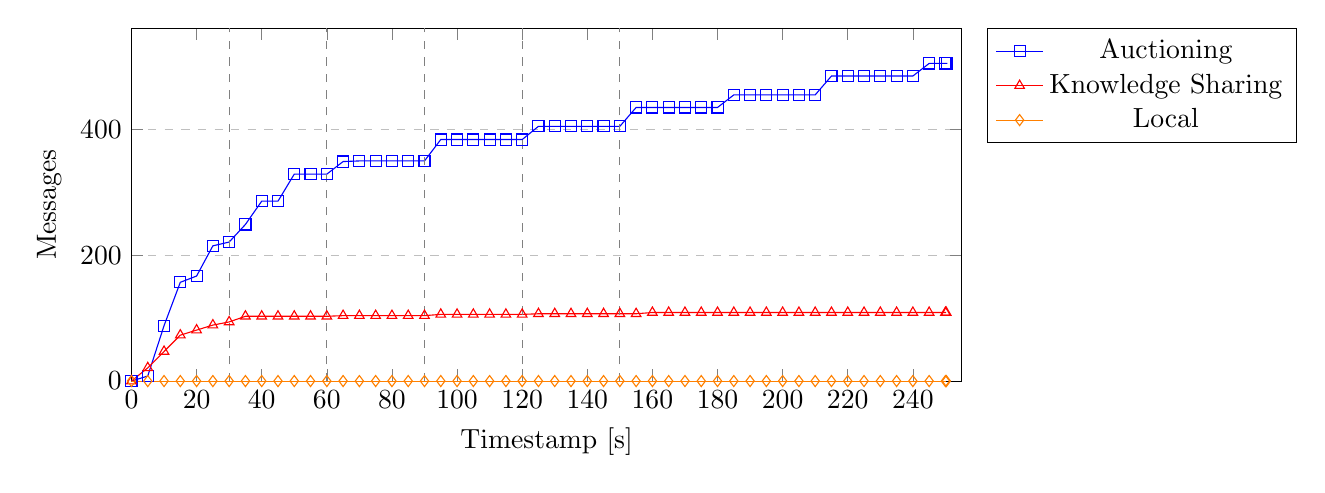
\begin{tikzpicture}
\begin{axis}[
    xlabel={Timestamp [s]},
    ylabel={Messages},
    xmin=0, xmax=255000,
    ymin=0, ymax=561,
    legend pos=outer north east,
    ymajorgrids=true,
    grid style=dashed,
    width=\textwidth,
    height=0.5\textwidth,
    scaled x ticks=base 10:-3,
    xtick scale label code/.code={}
]

	\addplot[color=blue,mark=square] coordinates {
        (0,0)(5000,8)(10000,88)(15000,157)(20000,167)(25000,215)(30000,221)(35000,249)(40000,286)(45000,286)(50000,329)(55000,329)(60000,329)(65000,349)(70000,350)(75000,350)(80000,350)(85000,350)(90000,350)(95000,384)(100000,384)(105000,384)(110000,384)(115000,384)(120000,384)(125000,405)(130000,405)(135000,405)(140000,405)(145000,405)(150000,405)(155000,435)(160000,435)(165000,435)(170000,435)(175000,435)(180000,435)(185000,455)(190000,455)(195000,455)(200000,455)(205000,455)(210000,455)(215000,485)(220000,485)(225000,485)(230000,485)(235000,485)(240000,485)(245000,505)(250000,505)(250569,505)
    };
    \addlegendentry{Auctioning}
	\addplot[color=red,mark=triangle] coordinates {
        (0,0)(5000,21)(10000,47)(15000,73)(20000,81)(25000,89)(30000,94)(35000,103)(40000,103)(45000,103)(50000,103)(55000,103)(60000,103)(65000,104)(70000,104)(75000,104)(80000,104)(85000,104)(90000,104)(95000,106)(100000,106)(105000,106)(110000,106)(115000,106)(120000,106)(125000,107)(130000,107)(135000,107)(140000,107)(145000,107)(150000,107)(155000,107)(160000,109)(165000,109)(170000,109)(175000,109)(180000,109)(185000,109)(190000,109)(195000,109)(200000,109)(205000,109)(210000,109)(215000,109)(220000,109)(225000,109)(230000,109)(235000,109)(240000,109)(245000,109)(250000,109)(250242,109)
    };
    \addlegendentry{Knowledge Sharing}
	\addplot[color=orange,mark=diamond] coordinates {
        (0,0)(5000,0)(10000,0)(15000,0)(20000,0)(25000,0)(30000,0)(35000,0)(40000,0)(45000,0)(50000,0)(55000,0)(60000,0)(65000,0)(70000,0)(75000,0)(80000,0)(85000,0)(90000,0)(95000,0)(100000,0)(105000,0)(110000,0)(115000,0)(120000,0)(125000,0)(130000,0)(135000,0)(140000,0)(145000,0)(150000,0)(155000,0)(160000,0)(165000,0)(170000,0)(175000,0)(180000,0)(185000,0)(190000,0)(195000,0)(200000,0)(205000,0)(210000,0)(215000,0)(220000,0)(225000,0)(230000,0)(235000,0)(240000,0)(245000,0)(250000,0)(250282,0)
    };
    \addlegendentry{Local}

	\addplot[color=gray, dashed,] coordinates {(30000,0) (30000,561)};
	\addplot[color=gray, dashed,] coordinates {(60000,0) (60000,561)};
	\addplot[color=gray, dashed,] coordinates {(90000,0) (90000,561)};
	\addplot[color=gray, dashed,] coordinates {(120000,0) (120000,561)};
	\addplot[color=gray, dashed,] coordinates {(150000,0) (150000,561)};


\end{axis}
\end{tikzpicture}
    \caption{Graph showing the total amount of messages sent between agents in the growing infrastructure scenario.}
\end{figure}
\begin{figure}[H]
    \centering
    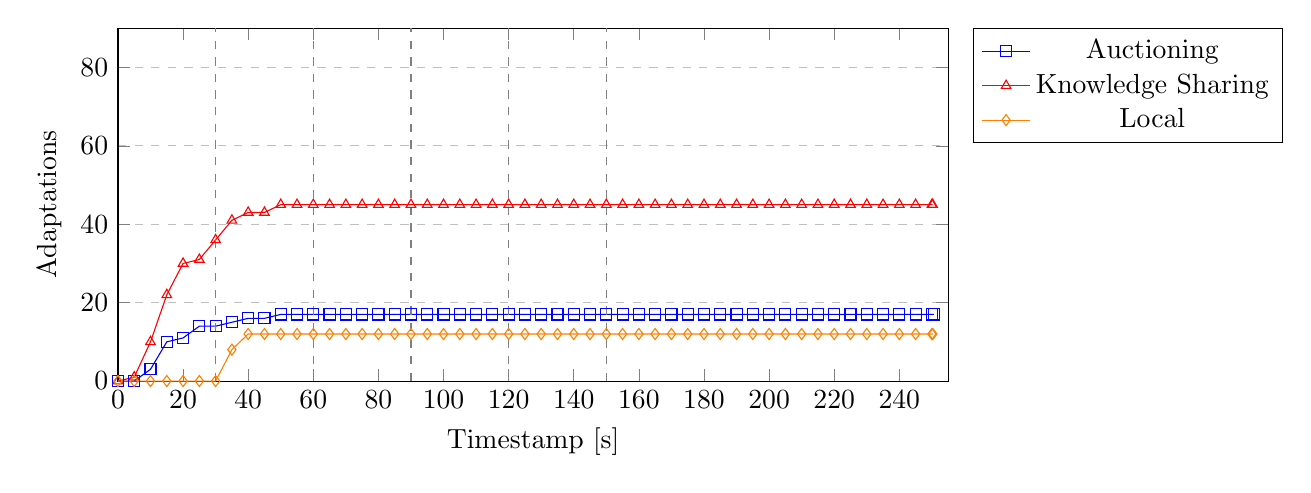
\begin{tikzpicture}
\begin{axis}[
    xlabel={Timestamp [s]},
    ylabel={Adaptations},
    xmin=0, xmax=255000,
    ymin=0, ymax=90,
    legend pos=outer north east,
    ymajorgrids=true,
    grid style=dashed,
    width=\textwidth,
    height=0.5\textwidth,
    scaled x ticks=base 10:-3,
    xtick scale label code/.code={}
]

	\addplot[color=blue,mark=square] coordinates {
        (0,0)(5000,0)(10000,3)(15000,10)(20000,11)(25000,14)(30000,14)(35000,15)(40000,16)(45000,16)(50000,17)(55000,17)(60000,17)(65000,17)(70000,17)(75000,17)(80000,17)(85000,17)(90000,17)(95000,17)(100000,17)(105000,17)(110000,17)(115000,17)(120000,17)(125000,17)(130000,17)(135000,17)(140000,17)(145000,17)(150000,17)(155000,17)(160000,17)(165000,17)(170000,17)(175000,17)(180000,17)(185000,17)(190000,17)(195000,17)(200000,17)(205000,17)(210000,17)(215000,17)(220000,17)(225000,17)(230000,17)(235000,17)(240000,17)(245000,17)(250000,17)(250569,17)
    };
    \addlegendentry{Auctioning}
	\addplot[color=red,mark=triangle] coordinates {
        (0,0)(5000,1)(10000,10)(15000,22)(20000,30)(25000,31)(30000,36)(35000,41)(40000,43)(45000,43)(50000,45)(55000,45)(60000,45)(65000,45)(70000,45)(75000,45)(80000,45)(85000,45)(90000,45)(95000,45)(100000,45)(105000,45)(110000,45)(115000,45)(120000,45)(125000,45)(130000,45)(135000,45)(140000,45)(145000,45)(150000,45)(155000,45)(160000,45)(165000,45)(170000,45)(175000,45)(180000,45)(185000,45)(190000,45)(195000,45)(200000,45)(205000,45)(210000,45)(215000,45)(220000,45)(225000,45)(230000,45)(235000,45)(240000,45)(245000,45)(250000,45)(250242,45)
    };
    \addlegendentry{Knowledge Sharing}
	\addplot[color=orange,mark=diamond] coordinates {
        (0,0)(5000,0)(10000,0)(15000,0)(20000,0)(25000,0)(30000,0)(35000,8)(40000,12)(45000,12)(50000,12)(55000,12)(60000,12)(65000,12)(70000,12)(75000,12)(80000,12)(85000,12)(90000,12)(95000,12)(100000,12)(105000,12)(110000,12)(115000,12)(120000,12)(125000,12)(130000,12)(135000,12)(140000,12)(145000,12)(150000,12)(155000,12)(160000,12)(165000,12)(170000,12)(175000,12)(180000,12)(185000,12)(190000,12)(195000,12)(200000,12)(205000,12)(210000,12)(215000,12)(220000,12)(225000,12)(230000,12)(235000,12)(240000,12)(245000,12)(250000,12)(250282,12)
    };
    \addlegendentry{Local}

	\addplot[color=gray, dashed,] coordinates {(30000,0) (30000,90)};
	\addplot[color=gray, dashed,] coordinates {(60000,0) (60000,90)};
	\addplot[color=gray, dashed,] coordinates {(90000,0) (90000,90)};
	\addplot[color=gray, dashed,] coordinates {(120000,0) (120000,90)};
	\addplot[color=gray, dashed,] coordinates {(150000,0) (150000,90)};


\end{axis}
\end{tikzpicture}
    \caption{Graph showing the total amount of adaptations applied by agents in the growing scenario.}
\end{figure}
\begin{figure}[H]
    \centering
        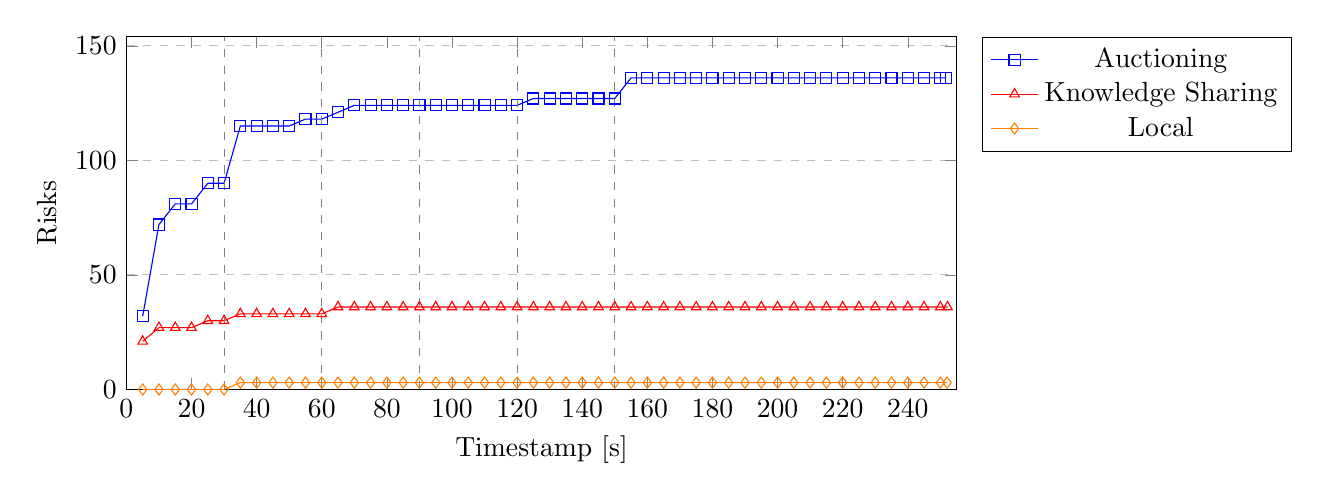
\begin{tikzpicture}
\begin{axis}[
    xlabel={Timestamp [s]},
    ylabel={Risks},
    xmin=0, xmax=255000,
    ymin=0, ymax=154,
    legend pos=outer north east,
    ymajorgrids=true,
    grid style=dashed,
    width=\textwidth,
    height=0.5\textwidth,
    scaled x ticks=base 10:-3,
    xtick scale label code/.code={}
]

	\addplot[color=blue,mark=square] coordinates {
        (5000,32)(10000,72)(15000,81)(20000,81)(25000,90)(30000,90)(35000,115)(40000,115)(45000,115)(50000,115)(55000,118)(60000,118)(65000,121)(70000,124)(75000,124)(80000,124)(85000,124)(90000,124)(95000,124)(100000,124)(105000,124)(110000,124)(115000,124)(120000,124)(125000,127)(130000,127)(135000,127)(140000,127)(145000,127)(150000,127)(155000,136)(160000,136)(165000,136)(170000,136)(175000,136)(180000,136)(185000,136)(190000,136)(195000,136)(200000,136)(205000,136)(210000,136)(215000,136)(220000,136)(225000,136)(230000,136)(235000,136)(240000,136)(245000,136)(250000,136)(251808,136)
    };
    \addlegendentry{Auctioning}
	\addplot[color=red,mark=triangle] coordinates {
        (5000,21)(10000,27)(15000,27)(20000,27)(25000,30)(30000,30)(35000,33)(40000,33)(45000,33)(50000,33)(55000,33)(60000,33)(65000,36)(70000,36)(75000,36)(80000,36)(85000,36)(90000,36)(95000,36)(100000,36)(105000,36)(110000,36)(115000,36)(120000,36)(125000,36)(130000,36)(135000,36)(140000,36)(145000,36)(150000,36)(155000,36)(160000,36)(165000,36)(170000,36)(175000,36)(180000,36)(185000,36)(190000,36)(195000,36)(200000,36)(205000,36)(210000,36)(215000,36)(220000,36)(225000,36)(230000,36)(235000,36)(240000,36)(245000,36)(250000,36)(252200,36)
    };
    \addlegendentry{Knowledge Sharing}
	\addplot[color=orange,mark=diamond] coordinates {
        (5000,0)(10000,0)(15000,0)(20000,0)(25000,0)(30000,0)(35000,3)(40000,3)(45000,3)(50000,3)(55000,3)(60000,3)(65000,3)(70000,3)(75000,3)(80000,3)(85000,3)(90000,3)(95000,3)(100000,3)(105000,3)(110000,3)(115000,3)(120000,3)(125000,3)(130000,3)(135000,3)(140000,3)(145000,3)(150000,3)(155000,3)(160000,3)(165000,3)(170000,3)(175000,3)(180000,3)(185000,3)(190000,3)(195000,3)(200000,3)(205000,3)(210000,3)(215000,3)(220000,3)(225000,3)(230000,3)(235000,3)(240000,3)(245000,3)(250000,3)(252076,3)
    };
    \addlegendentry{Local}

	\addplot[color=gray, dashed,] coordinates {(30000,0) (30000,154)};
	\addplot[color=gray, dashed,] coordinates {(60000,0) (60000,154)};
	\addplot[color=gray, dashed,] coordinates {(90000,0) (90000,154)};
	\addplot[color=gray, dashed,] coordinates {(120000,0) (120000,154)};
	\addplot[color=gray, dashed,] coordinates {(150000,0) (150000,154)};


\end{axis}
\end{tikzpicture}
    \caption{Graph showing the number of unique risks detected by agents in the growing scenario.}
\end{figure}
\begin{figure}[H]
    \centering
        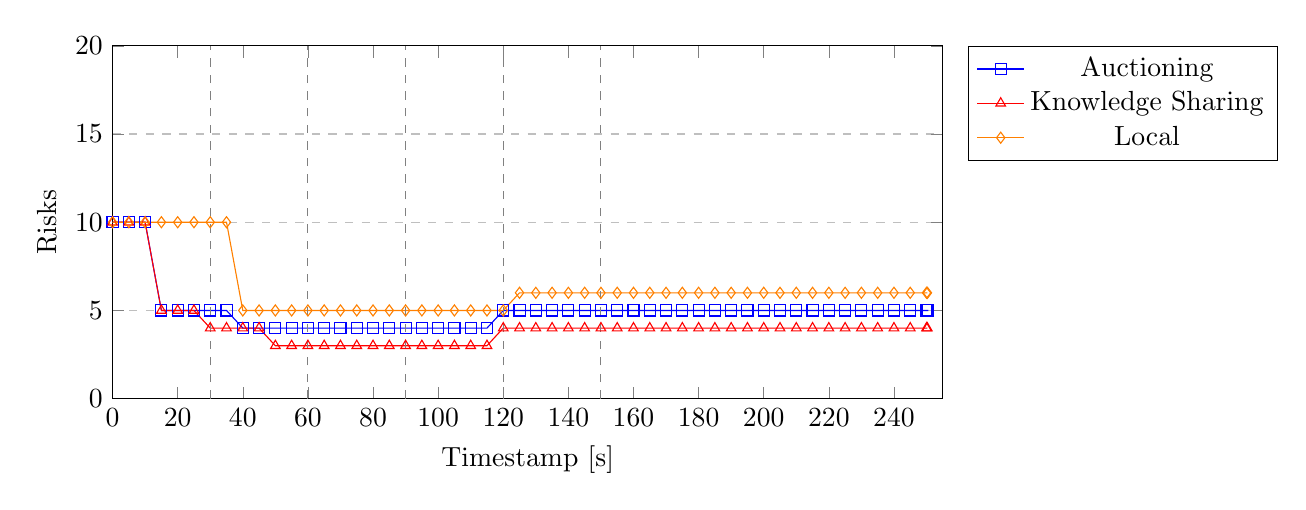
\begin{tikzpicture}
\begin{axis}[
    xlabel={Timestamp [s]},
    ylabel={Risks},
    xmin=0, xmax=255000,
    ymin=0, ymax=20,
    legend pos=outer north east,
    ymajorgrids=true,
    grid style=dashed,
    width=\textwidth,
    height=0.5\textwidth,
    scaled x ticks=base 10:-3,
    xtick scale label code/.code={}
]

	\addplot[color=blue,mark=square] coordinates {
        (0,10)(5000,10)(10000,10)(15000,5)(20000,5)(25000,5)(30000,5)(35000,5)(40000,4)(45000,4)(50000,4)(55000,4)(60000,4)(65000,4)(70000,4)(75000,4)(80000,4)(85000,4)(90000,4)(95000,4)(100000,4)(105000,4)(110000,4)(115000,4)(120000,5)(125000,5)(130000,5)(135000,5)(140000,5)(145000,5)(150000,5)(155000,5)(160000,5)(165000,5)(170000,5)(175000,5)(180000,5)(185000,5)(190000,5)(195000,5)(200000,5)(205000,5)(210000,5)(215000,5)(220000,5)(225000,5)(230000,5)(235000,5)(240000,5)(245000,5)(250000,5)(250569,5)
    };
    \addlegendentry{Auctioning}
	\addplot[color=red,mark=triangle] coordinates {
        (0,10)(5000,10)(10000,10)(15000,5)(20000,5)(25000,5)(30000,4)(35000,4)(40000,4)(45000,4)(50000,3)(55000,3)(60000,3)(65000,3)(70000,3)(75000,3)(80000,3)(85000,3)(90000,3)(95000,3)(100000,3)(105000,3)(110000,3)(115000,3)(120000,4)(125000,4)(130000,4)(135000,4)(140000,4)(145000,4)(150000,4)(155000,4)(160000,4)(165000,4)(170000,4)(175000,4)(180000,4)(185000,4)(190000,4)(195000,4)(200000,4)(205000,4)(210000,4)(215000,4)(220000,4)(225000,4)(230000,4)(235000,4)(240000,4)(245000,4)(250000,4)(250242,4)
    };
    \addlegendentry{Knowledge Sharing}
	\addplot[color=orange,mark=diamond] coordinates {
        (0,10)(5000,10)(10000,10)(15000,10)(20000,10)(25000,10)(30000,10)(35000,10)(40000,5)(45000,5)(50000,5)(55000,5)(60000,5)(65000,5)(70000,5)(75000,5)(80000,5)(85000,5)(90000,5)(95000,5)(100000,5)(105000,5)(110000,5)(115000,5)(120000,5)(125000,6)(130000,6)(135000,6)(140000,6)(145000,6)(150000,6)(155000,6)(160000,6)(165000,6)(170000,6)(175000,6)(180000,6)(185000,6)(190000,6)(195000,6)(200000,6)(205000,6)(210000,6)(215000,6)(220000,6)(225000,6)(230000,6)(235000,6)(240000,6)(245000,6)(250000,6)(250282,6)
    };
    \addlegendentry{Local}

	\addplot[color=gray, dashed,] coordinates {(30000,0) (30000,20)};
	\addplot[color=gray, dashed,] coordinates {(60000,0) (60000,20)};
	\addplot[color=gray, dashed,] coordinates {(90000,0) (90000,20)};
	\addplot[color=gray, dashed,] coordinates {(120000,0) (120000,20)};
	\addplot[color=gray, dashed,] coordinates {(150000,0) (150000,20)};


\end{axis}
\end{tikzpicture}
    \caption{Graph showing the number of remaining risks in the infrastructure in the growing scenario.}
\end{figure}
\begin{figure}[H]
    \centering
        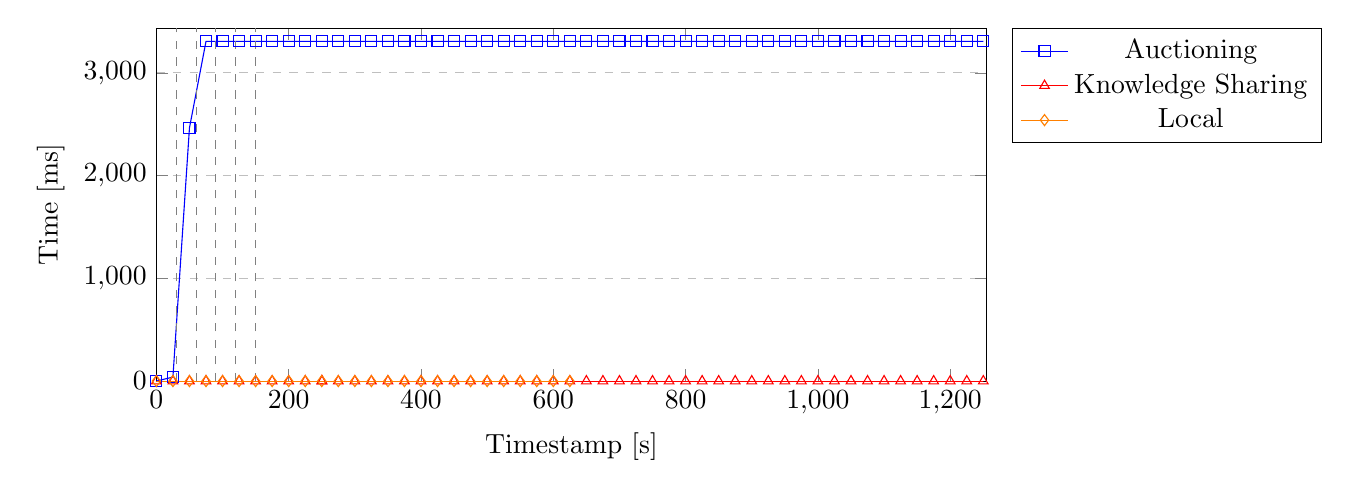
\begin{tikzpicture}
\begin{axis}[
    xlabel={Timestamp [s]},
    ylabel={Time [ms]},
    xmin=0, xmax=1255000,
    ymin=0, ymax=3434,
    legend pos=outer north east,
    ymajorgrids=true,
    grid style=dashed,
    width=\textwidth,
    height=0.5\textwidth,
    scaled x ticks=base 10:-3,
    xtick scale label code/.code={}
]

	\addplot[color=blue,mark=square] coordinates {
        (0,0)(25000,39)(50000,2464)(75000,3306)(100000,3306)(125000,3306)(150000,3306)(175000,3306)(200000,3306)(225000,3306)(250000,3306)(275000,3306)(300000,3306)(325000,3306)(350000,3306)(375000,3306)(400000,3306)(425000,3306)(450000,3306)(475000,3306)(500000,3306)(525000,3306)(550000,3306)(575000,3306)(600000,3306)(625000,3306)(650000,3306)(675000,3306)(700000,3306)(725000,3306)(750000,3306)(775000,3306)(800000,3306)(825000,3306)(850000,3306)(875000,3306)(900000,3306)(925000,3306)(950000,3306)(975000,3306)(1000000,3306)(1025000,3306)(1050000,3306)(1075000,3306)(1100000,3306)(1125000,3306)(1150000,3306)(1175000,3306)(1200000,3306)(1225000,3306)(1250000,3306)(250447,3306)
    };
    \addlegendentry{Auctioning}
	\addplot[color=red,mark=triangle] coordinates {
        (0,0)(25000,0)(50000,0)(75000,0)(100000,0)(125000,0)(150000,0)(175000,0)(200000,0)(225000,0)(250000,0)(275000,0)(300000,0)(325000,0)(350000,0)(375000,0)(400000,0)(425000,0)(450000,0)(475000,0)(500000,0)(525000,0)(550000,0)(575000,0)(600000,0)(625000,0)(650000,0)(675000,0)(700000,0)(725000,0)(750000,0)(775000,0)(800000,0)(825000,0)(850000,0)(875000,0)(900000,0)(925000,0)(950000,0)(975000,0)(1000000,0)(1025000,0)(1050000,0)(1075000,0)(1100000,0)(1125000,0)(1150000,0)(1175000,0)(1200000,0)(1225000,0)(1250000,0)(250418,0)
    };
    \addlegendentry{Knowledge Sharing}
	\addplot[color=orange,mark=diamond] coordinates {
        (0,0)(25000,0)(50000,0)(75000,0)(100000,0)(125000,0)(150000,0)(175000,0)(200000,0)(225000,0)(250000,0)(275000,0)(300000,0)(325000,0)(350000,0)(375000,0)(400000,0)(425000,0)(450000,0)(475000,0)(500000,0)(525000,0)(550000,0)(575000,0)(600000,0)(625000,0)
    };
    \addlegendentry{Local}

	\addplot[color=gray, dashed,] coordinates {(30000,0) (30000,3434)};
	\addplot[color=gray, dashed,] coordinates {(60000,0) (60000,3434)};
	\addplot[color=gray, dashed,] coordinates {(90000,0) (90000,3434)};
	\addplot[color=gray, dashed,] coordinates {(120000,0) (120000,3434)};
	\addplot[color=gray, dashed,] coordinates {(150000,0) (150000,3434)};


\end{axis}
\end{tikzpicture}
    \caption{Graph showing the sum of time spent auctioning by agents in the growing scenario.}
\end{figure}
\begin{figure}[H]
    \centering
        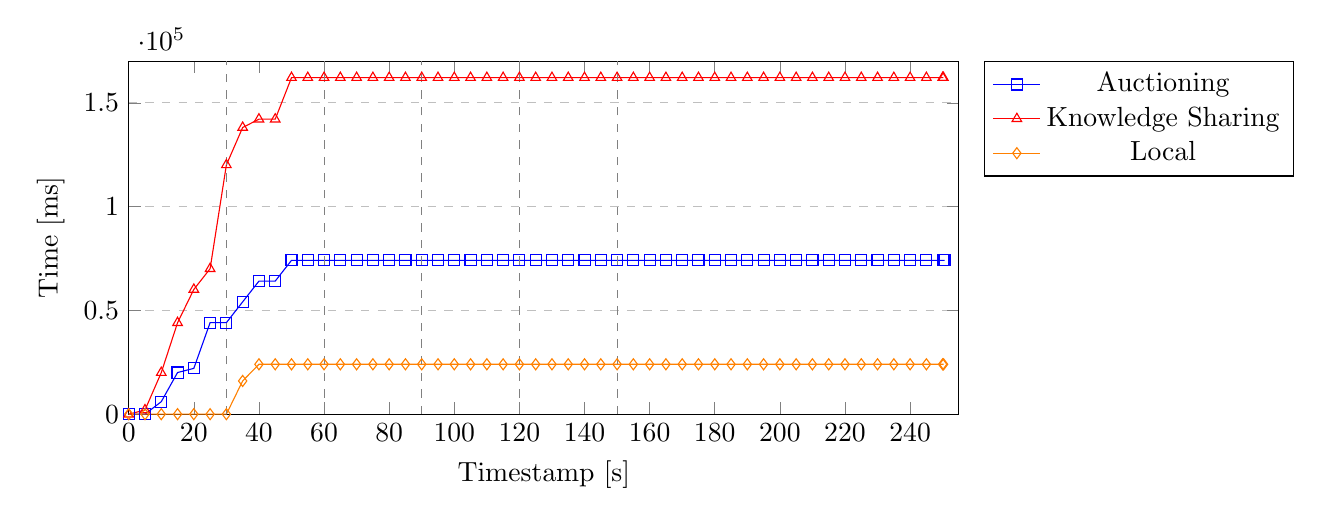
\begin{tikzpicture}
\begin{axis}[
    xlabel={Timestamp [s]},
    ylabel={Time [ms]},
    xmin=0, xmax=255000,
    ymin=0, ymax=170017,
    legend pos=outer north east,
    ymajorgrids=true,
    grid style=dashed,
    width=\textwidth,
    height=0.5\textwidth,
    scaled x ticks=base 10:-3,
    xtick scale label code/.code={}
]

	\addplot[color=blue,mark=square] coordinates {
        (0,0)(5000,0)(10000,6018)(15000,20071)(20000,22078)(25000,44102)(30000,44102)(35000,54111)(40000,64119)(45000,64119)(50000,74128)(55000,74128)(60000,74128)(65000,74128)(70000,74128)(75000,74128)(80000,74128)(85000,74128)(90000,74128)(95000,74128)(100000,74128)(105000,74128)(110000,74128)(115000,74128)(120000,74128)(125000,74128)(130000,74128)(135000,74128)(140000,74128)(145000,74128)(150000,74128)(155000,74128)(160000,74128)(165000,74128)(170000,74128)(175000,74128)(180000,74128)(185000,74128)(190000,74128)(195000,74128)(200000,74128)(205000,74128)(210000,74128)(215000,74128)(220000,74128)(225000,74128)(230000,74128)(235000,74128)(240000,74128)(245000,74128)(250000,74128)(250569,74128)
    };
    \addlegendentry{Auctioning}
	\addplot[color=red,mark=triangle] coordinates {
        (0,0)(5000,2004)(10000,20023)(15000,44059)(20000,60095)(25000,70097)(30000,120113)(35000,138132)(40000,142140)(45000,142140)(50000,162147)(55000,162147)(60000,162147)(65000,162147)(70000,162147)(75000,162147)(80000,162147)(85000,162147)(90000,162147)(95000,162147)(100000,162147)(105000,162147)(110000,162147)(115000,162147)(120000,162147)(125000,162147)(130000,162147)(135000,162147)(140000,162147)(145000,162147)(150000,162147)(155000,162147)(160000,162147)(165000,162147)(170000,162147)(175000,162147)(180000,162147)(185000,162147)(190000,162147)(195000,162147)(200000,162147)(205000,162147)(210000,162147)(215000,162147)(220000,162147)(225000,162147)(230000,162147)(235000,162147)(240000,162147)(245000,162147)(250000,162147)(250242,162147)
    };
    \addlegendentry{Knowledge Sharing}
	\addplot[color=orange,mark=diamond] coordinates {
        (0,0)(5000,0)(10000,0)(15000,0)(20000,0)(25000,0)(30000,0)(35000,16023)(40000,24038)(45000,24038)(50000,24038)(55000,24038)(60000,24038)(65000,24038)(70000,24038)(75000,24038)(80000,24038)(85000,24038)(90000,24038)(95000,24038)(100000,24038)(105000,24038)(110000,24038)(115000,24038)(120000,24038)(125000,24038)(130000,24038)(135000,24038)(140000,24038)(145000,24038)(150000,24038)(155000,24038)(160000,24038)(165000,24038)(170000,24038)(175000,24038)(180000,24038)(185000,24038)(190000,24038)(195000,24038)(200000,24038)(205000,24038)(210000,24038)(215000,24038)(220000,24038)(225000,24038)(230000,24038)(235000,24038)(240000,24038)(245000,24038)(250000,24038)(250282,24038)
    };
    \addlegendentry{Local}

	\addplot[color=gray, dashed,] coordinates {(30000,0) (30000,170017)};
	\addplot[color=gray, dashed,] coordinates {(60000,0) (60000,170017)};
	\addplot[color=gray, dashed,] coordinates {(90000,0) (90000,170017)};
	\addplot[color=gray, dashed,] coordinates {(120000,0) (120000,170017)};
	\addplot[color=gray, dashed,] coordinates {(150000,0) (150000,170017)};


\end{axis}
\end{tikzpicture}
    \caption{Graph showing the sum of time spent adapting by agents in the growing scenario.}
\end{figure}
